\documentclass{article}
\usepackage{pdfpages} % Required package for including PDFs
\usepackage{graphicx} % Required package for including images
\usepackage{hyperref} % Required for hyperlinks
\usepackage{lipsum}   % Used for generating dummy text (remove in your actual document)

\begin{document}

\title{EngMath - ps\_1}
\author{A. Q. Snyder}
\date{\today}

\maketitle

\section{HW template}

\noindent
For more details, the entire template and its supplementary materials can be found on GitHub: \href{https://github.com/aqsnyder/eng_math/tree/main/ps_1}{here}.
Under the ps\_1 directory exist the necessary files for this LaTeX generation, the compiled plots, MATLAB exports, Python exports, the virtual Jupyter kernels used to prototype Python code, and all MATLAB files.

\includepdf[pages=-]{misc_media/hw1_prompt.pdf}

\section{Hand Calcs}
\begin{figure}[h]
    \centering
    
\includegraphics[width=0.5\textwidth]{misc_media/hand-calcs.jpg}
    \caption{Hand Calculations} % Optional: add a caption
    \label{fig:hand-calcs}      % Optional: add a label for referencing
\end{figure}

\vspace{2cm}  % Add vertical space of 2cm

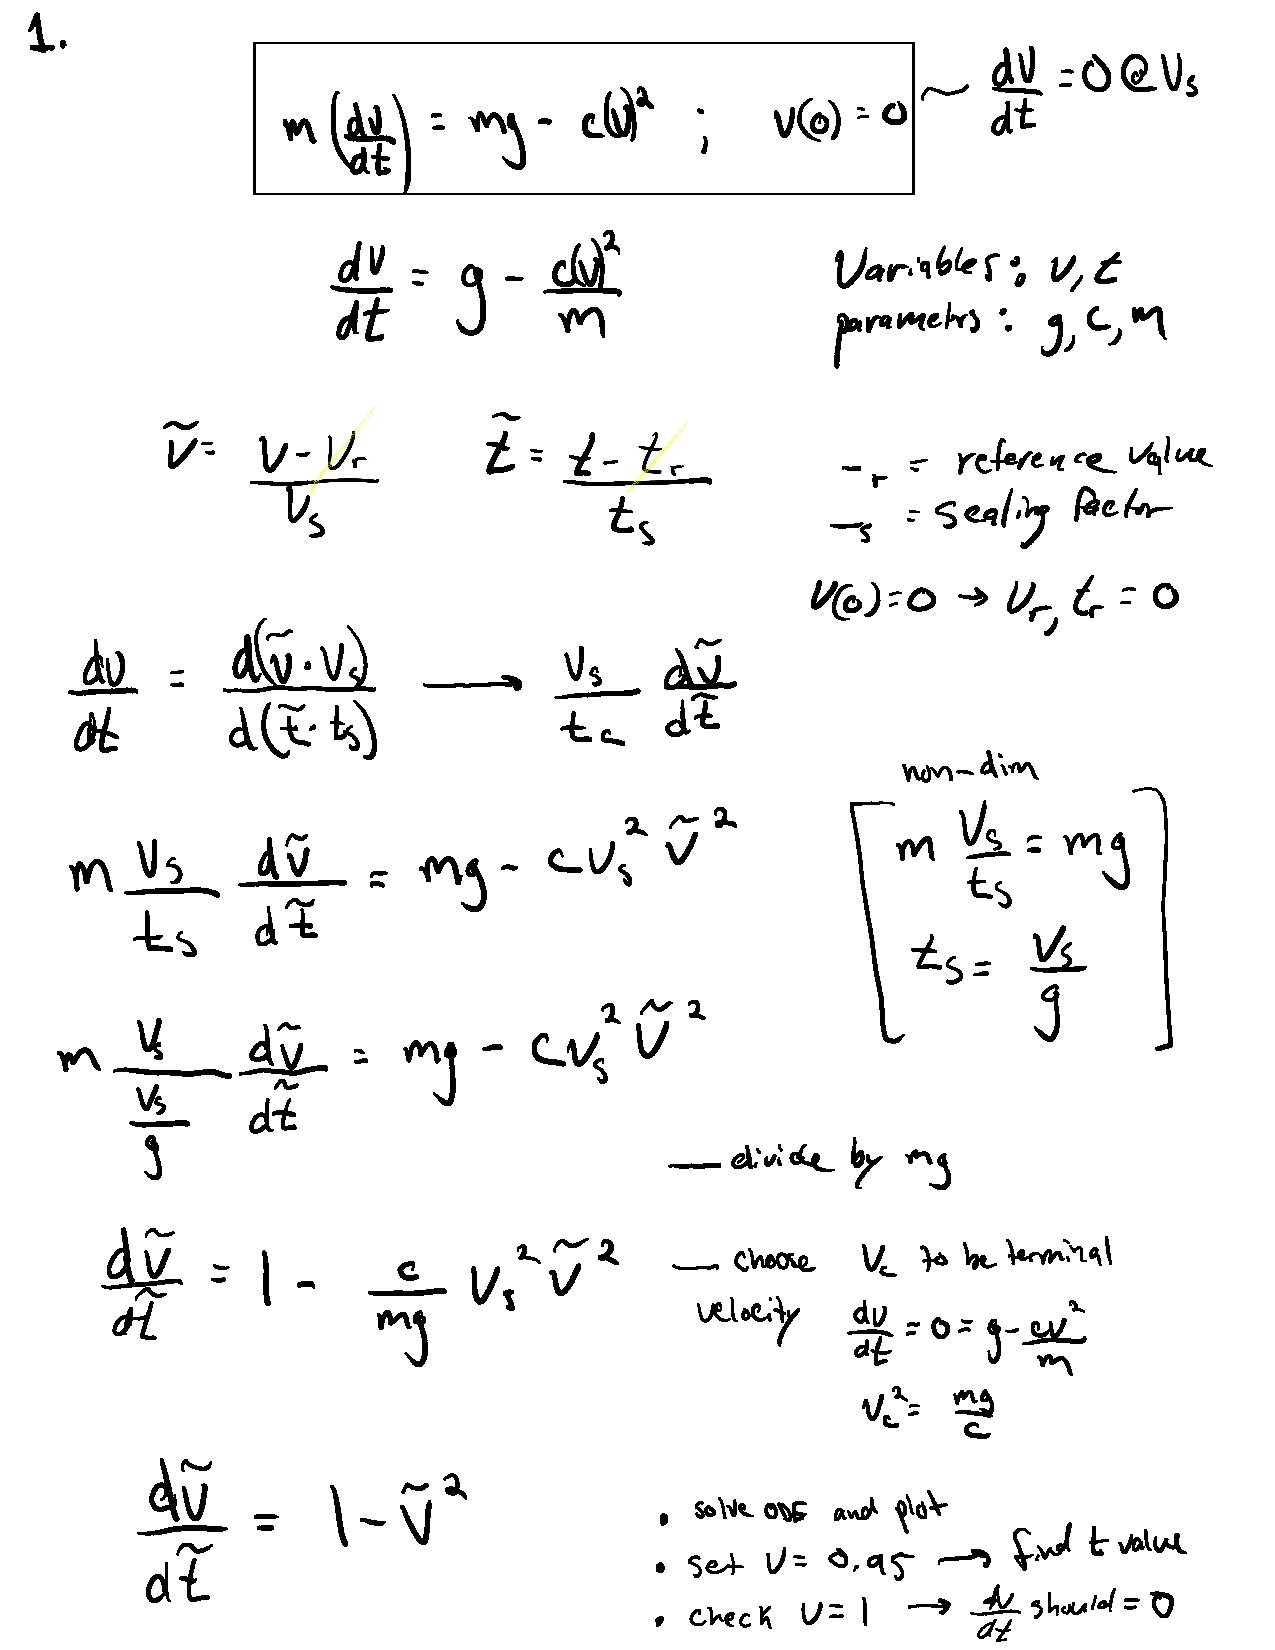
\includepdf[pages=-]{hand_calcs/problem_1.pdf} 
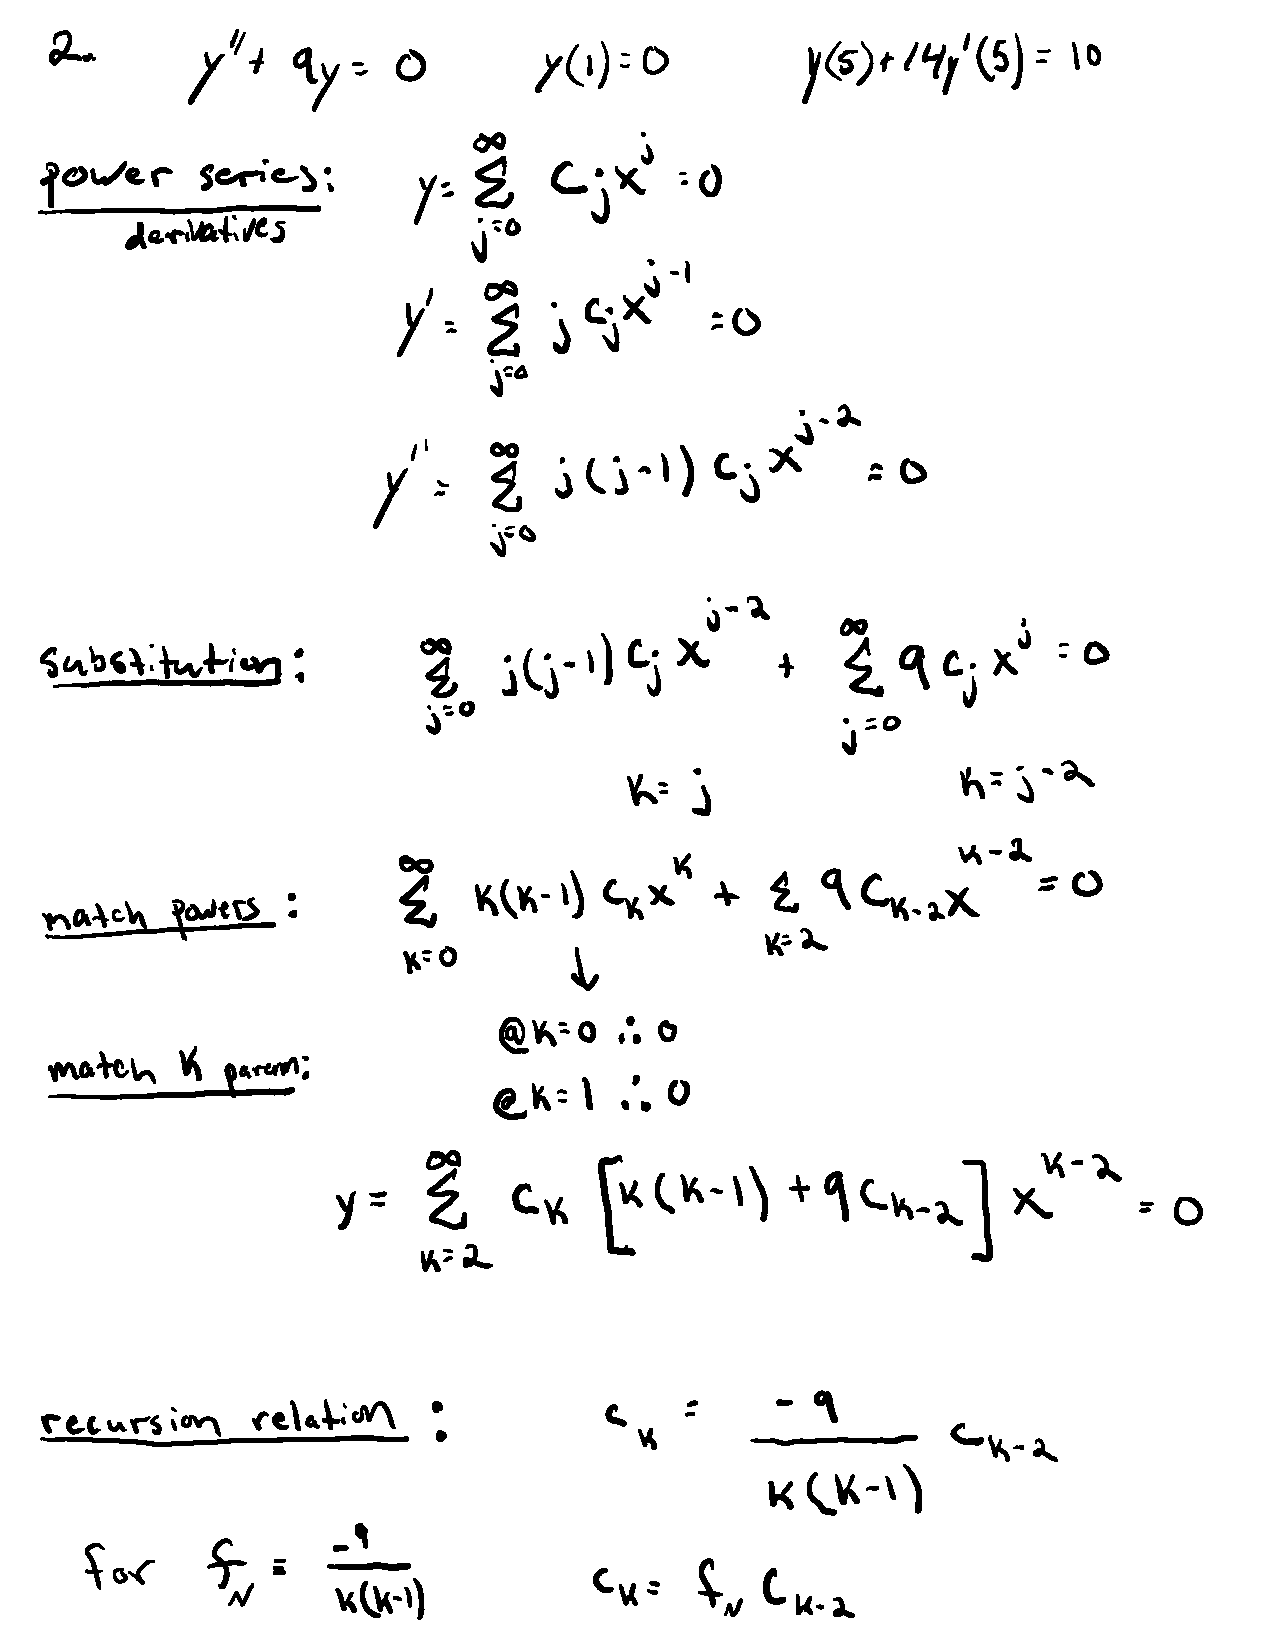
\includepdf[pages=-]{hand_calcs/problem_2.pdf} 
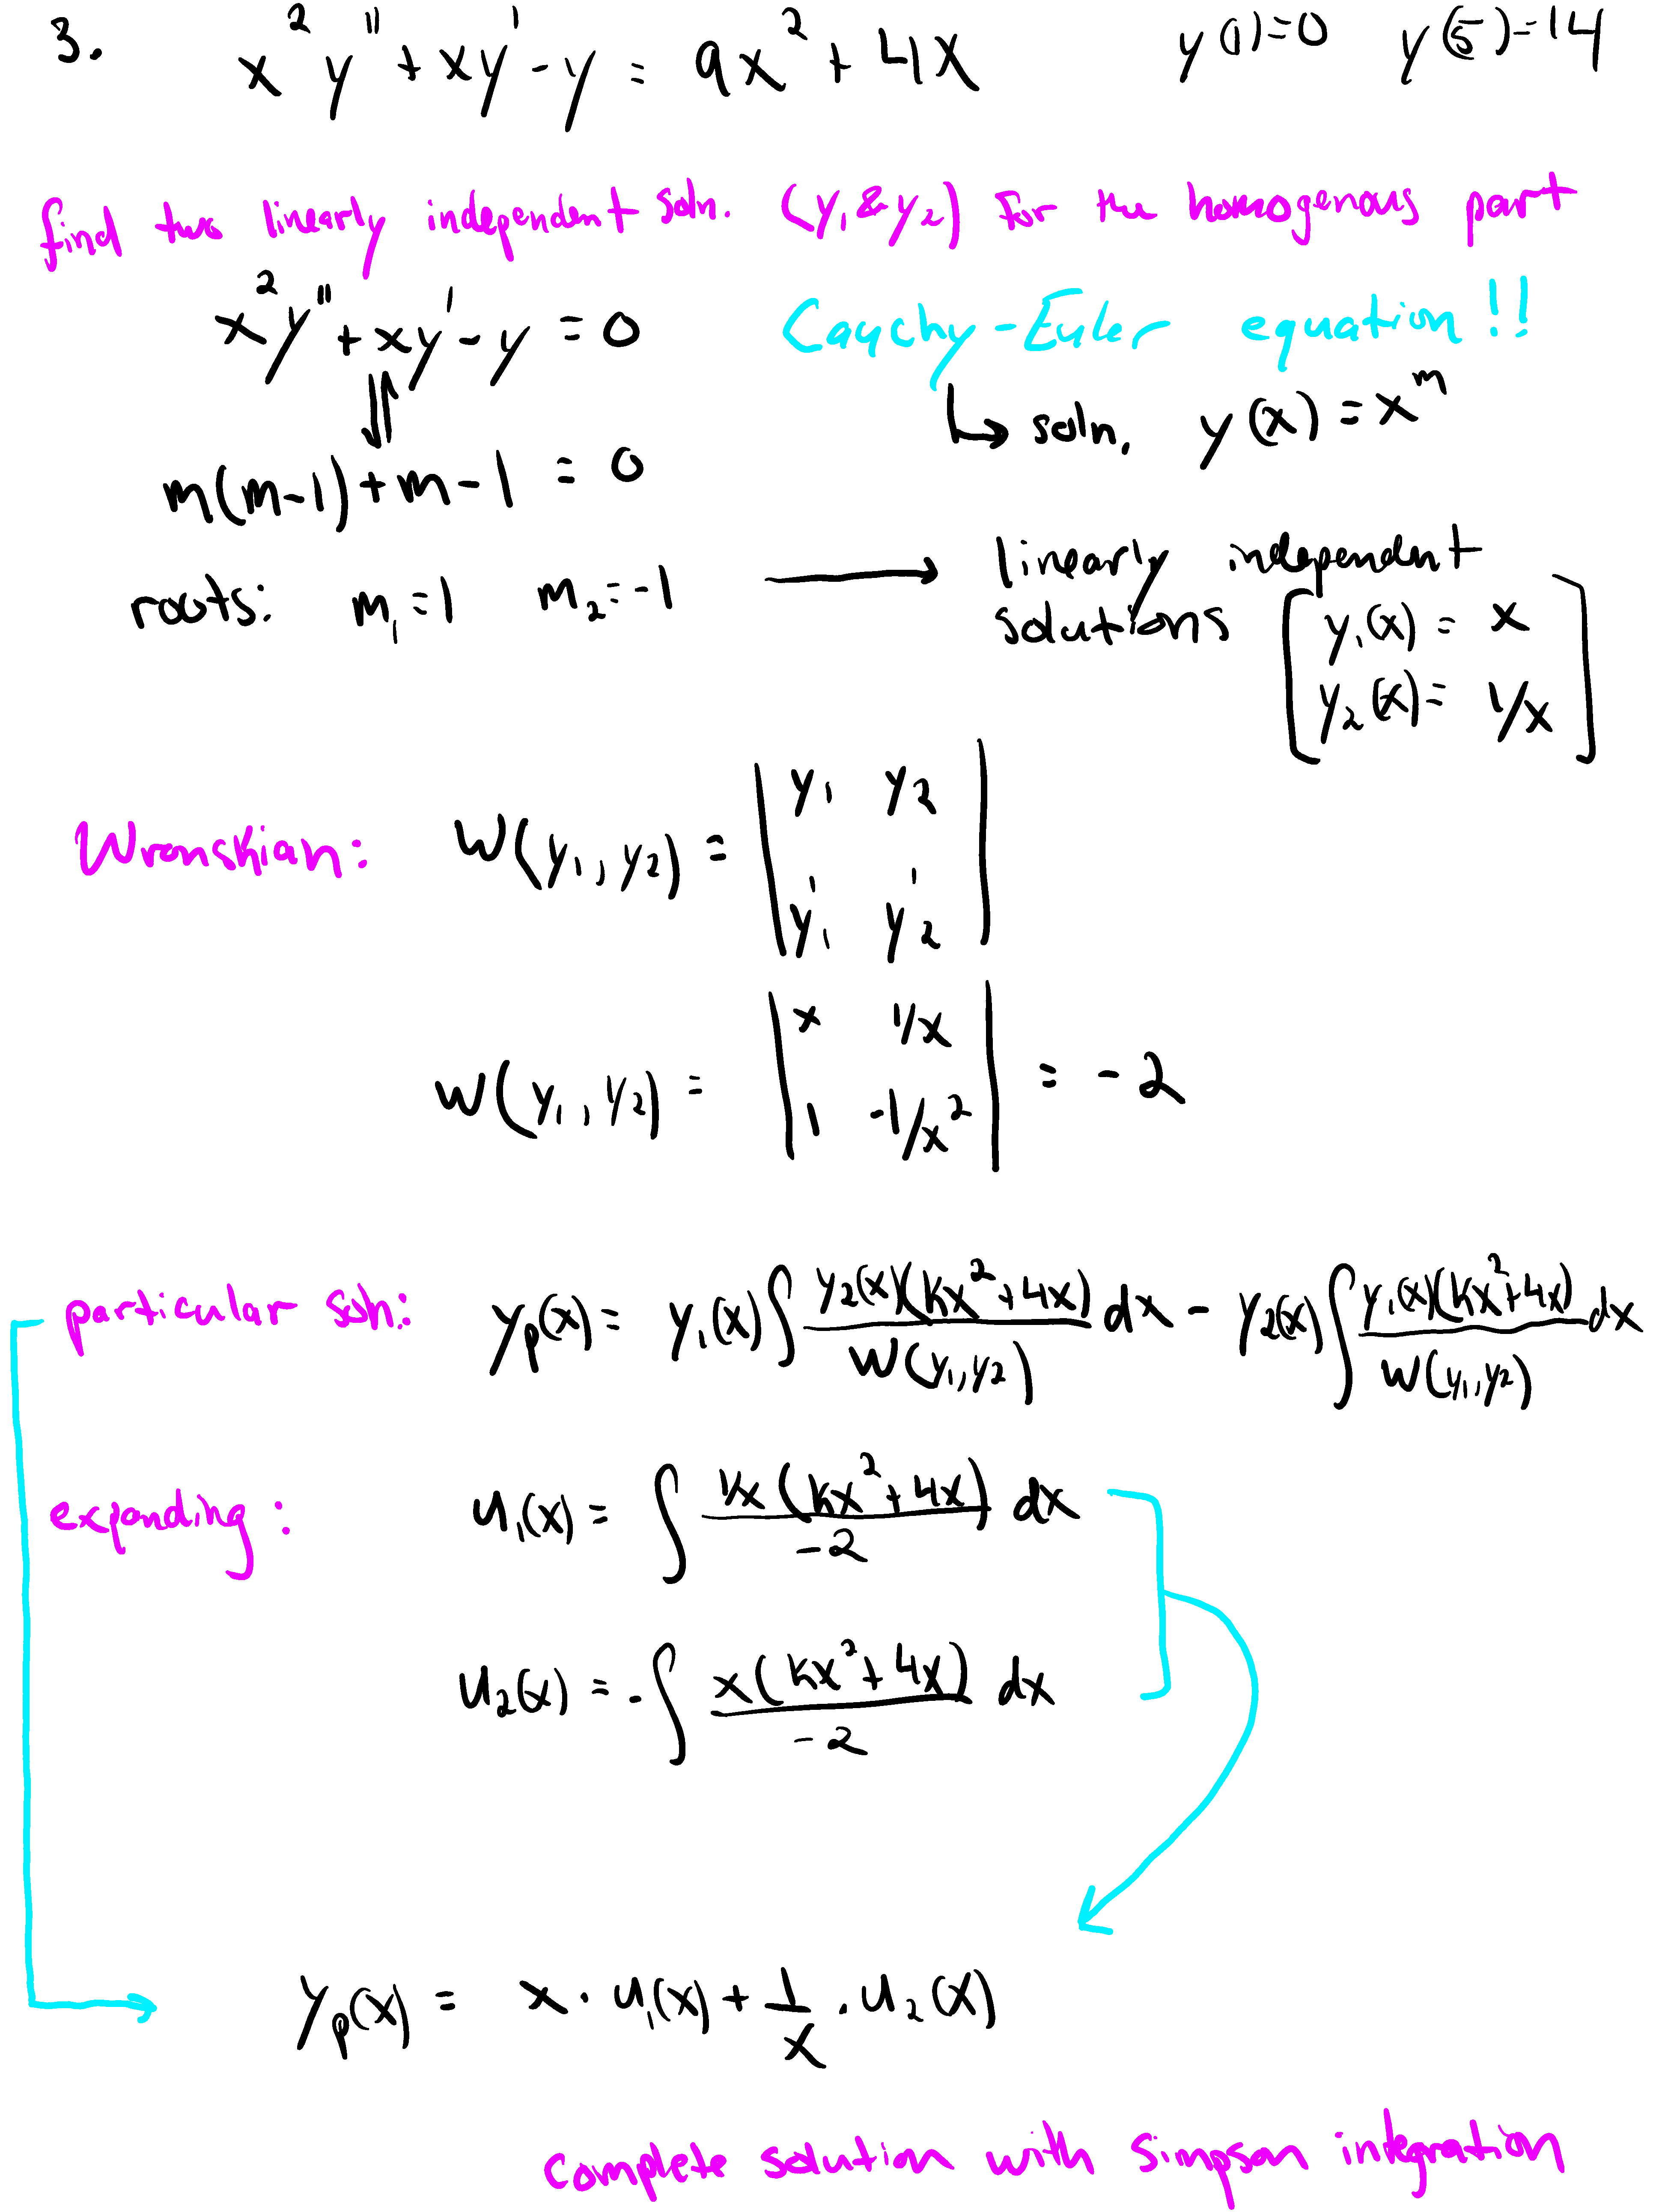
\includepdf[pages=-]{hand_calcs/problem_3.pdf} 
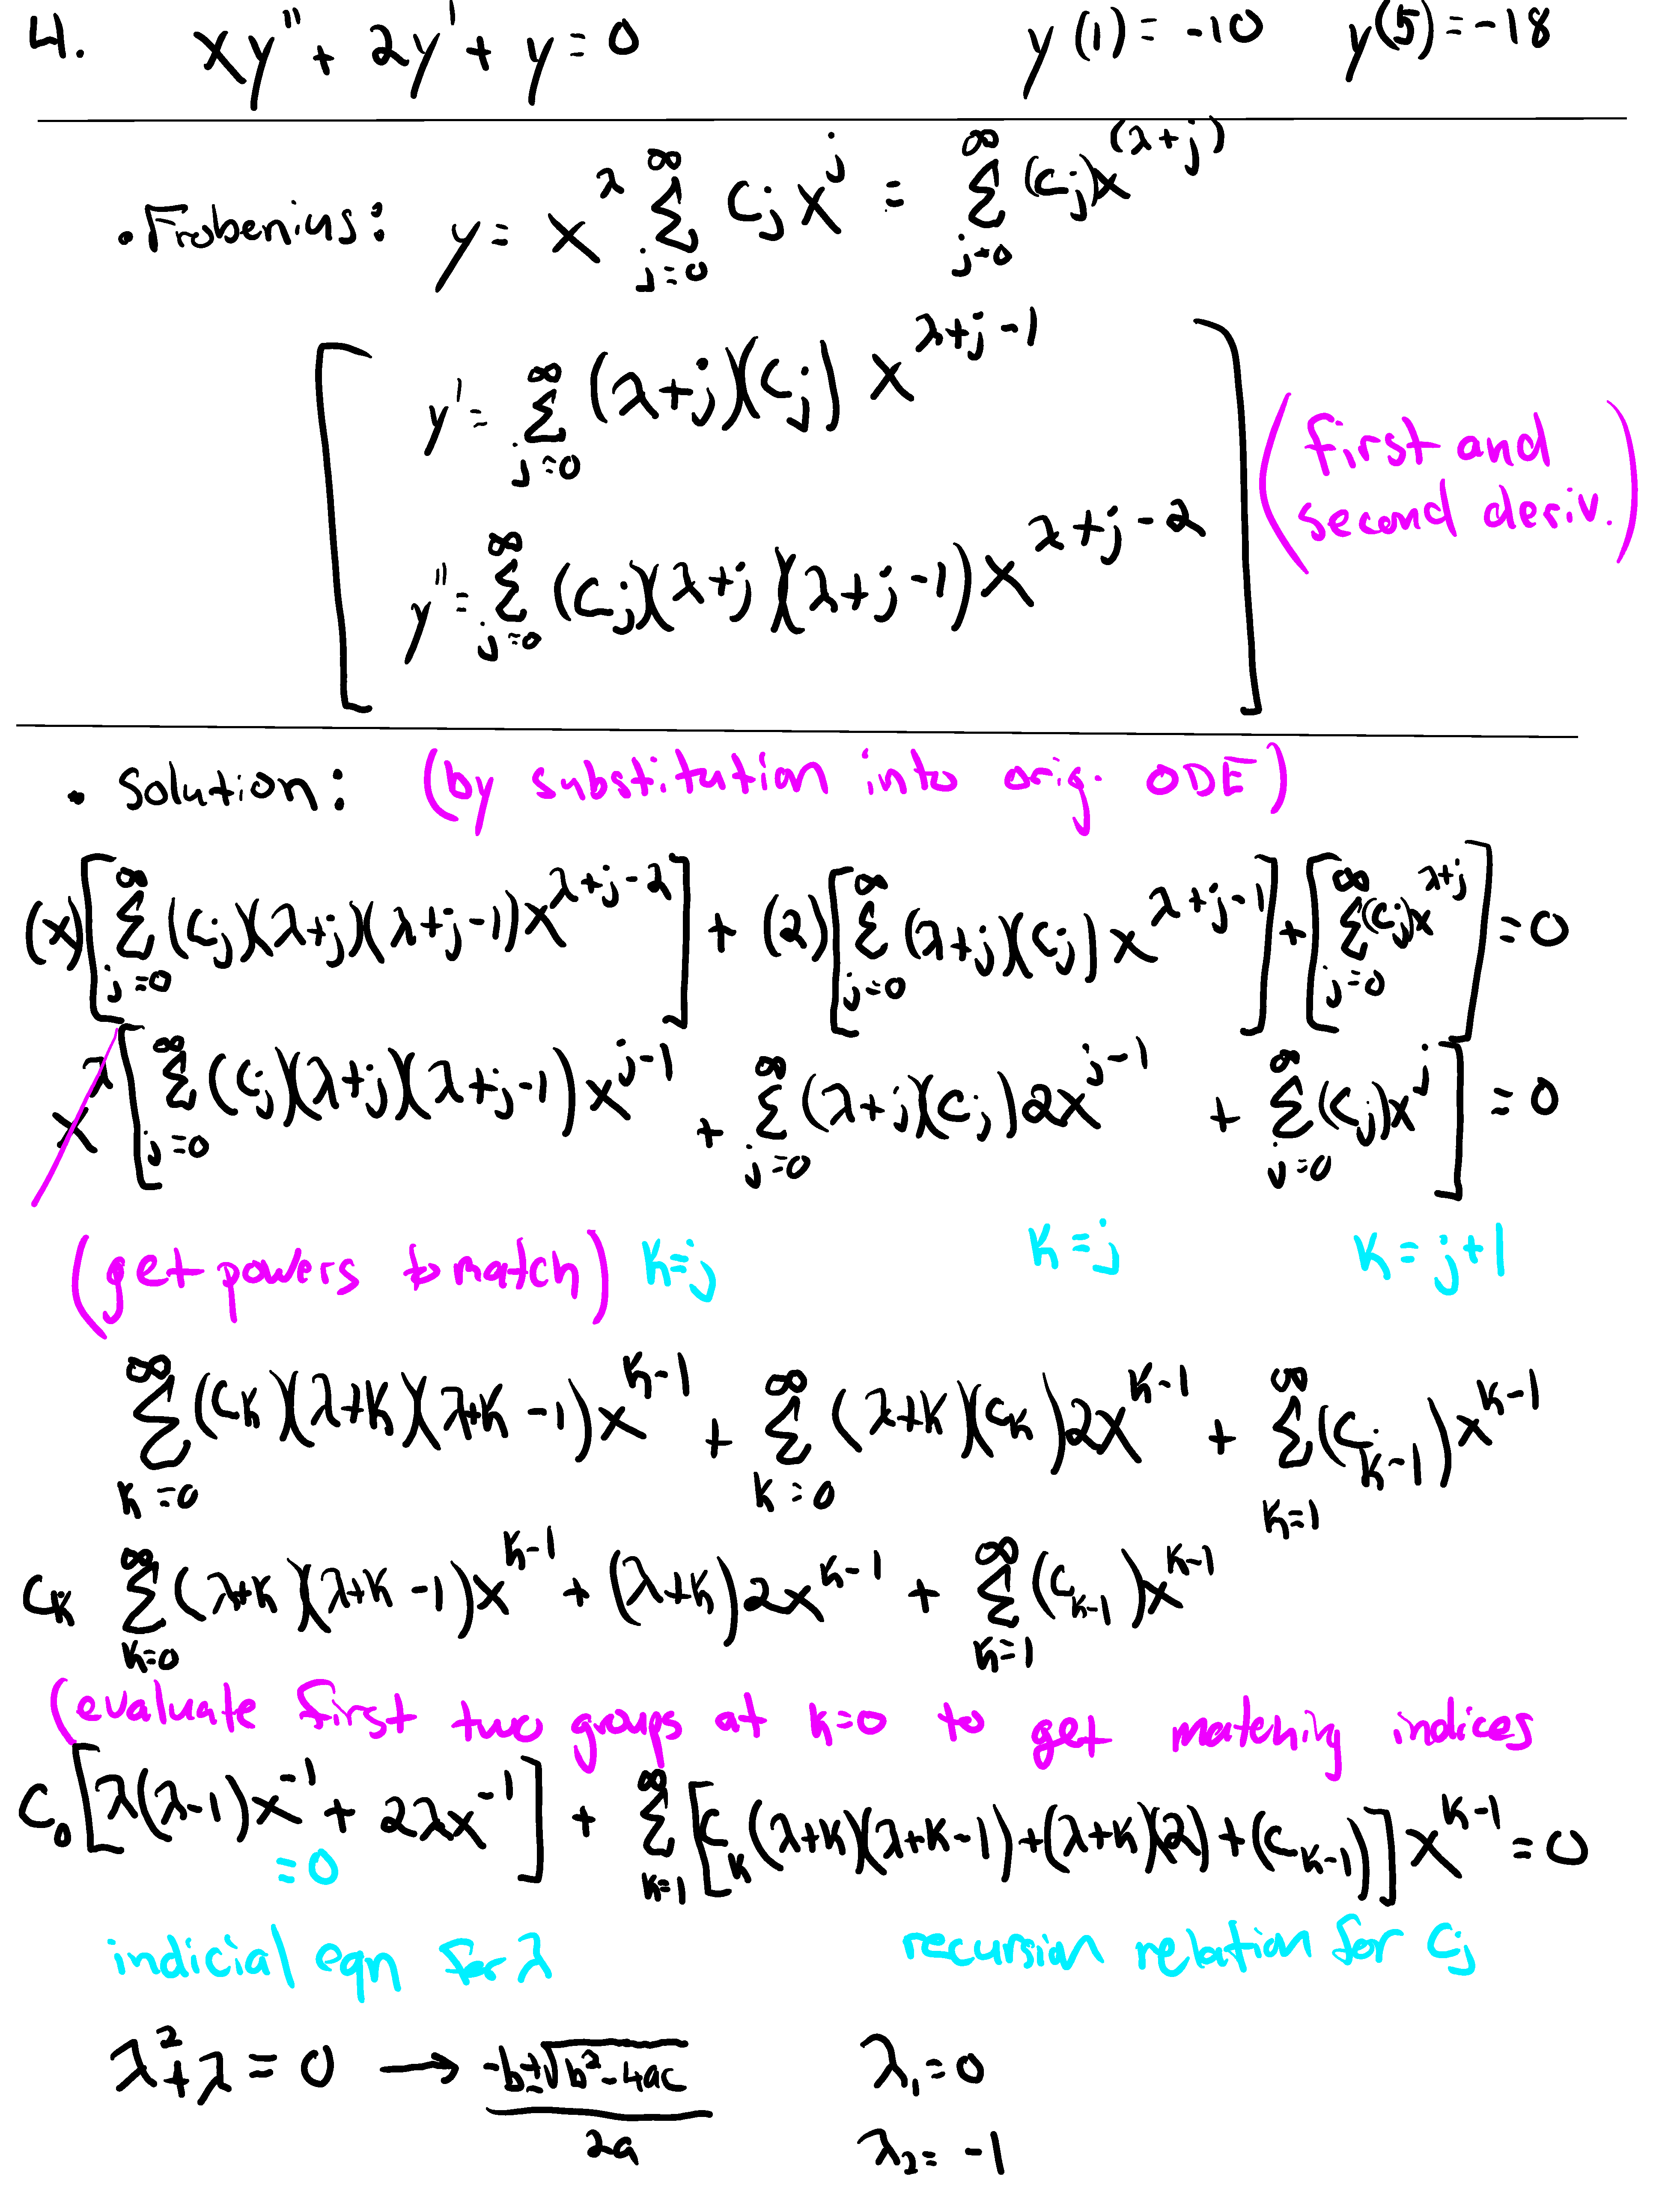
\includepdf[pages=-]{hand_calcs/problem_4.pdf} 

\section{Python Outputs}
\begin{figure}[h]
    \centering
    
\includegraphics[width=0.5\textwidth]{misc_media/Python-Logo.jpg}
    \caption{Python Logo}  % Optional: add a caption
    \label{fig:python-logo} % Optional: add a label for referencing
\end{figure}

\vspace{2cm}  % Add vertical space of 2cm

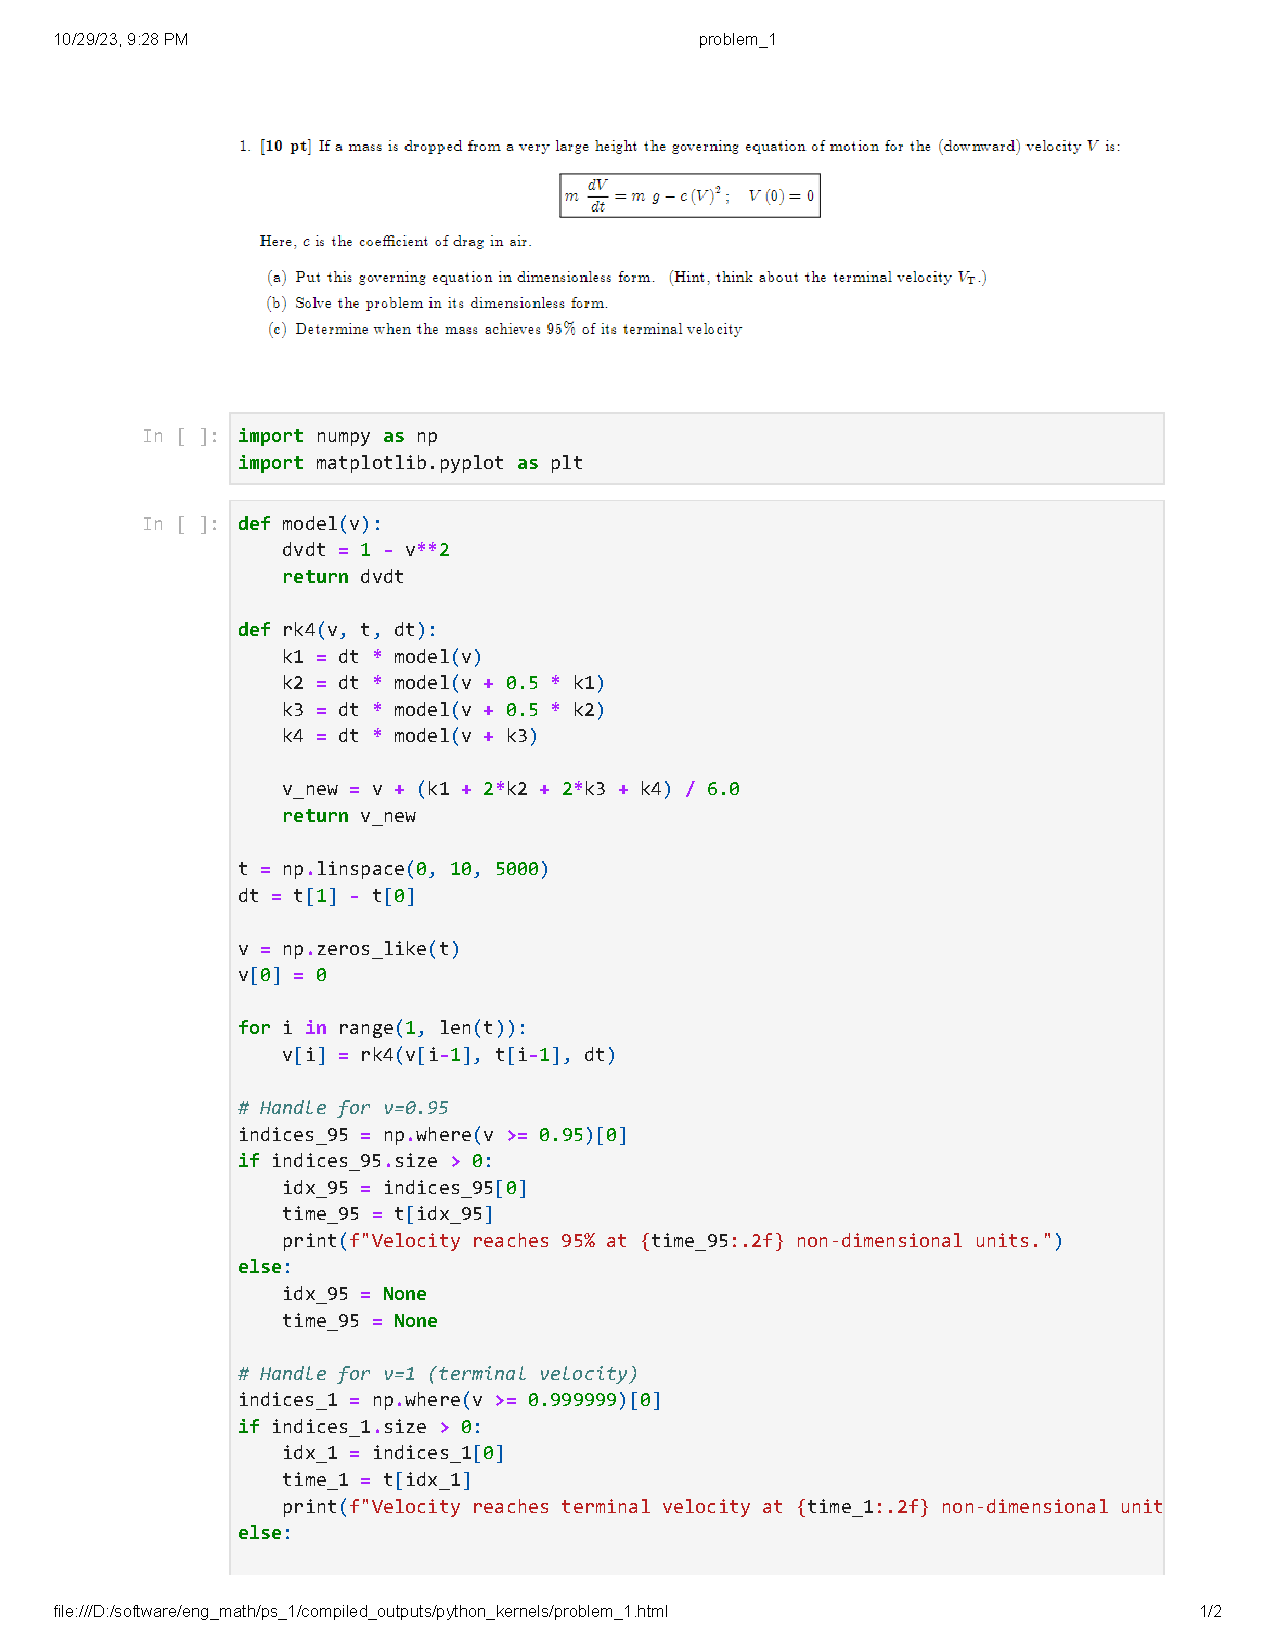
\includepdf[pages=-]{compiled_outputs/python_kernels/problem_1.pdf}
% 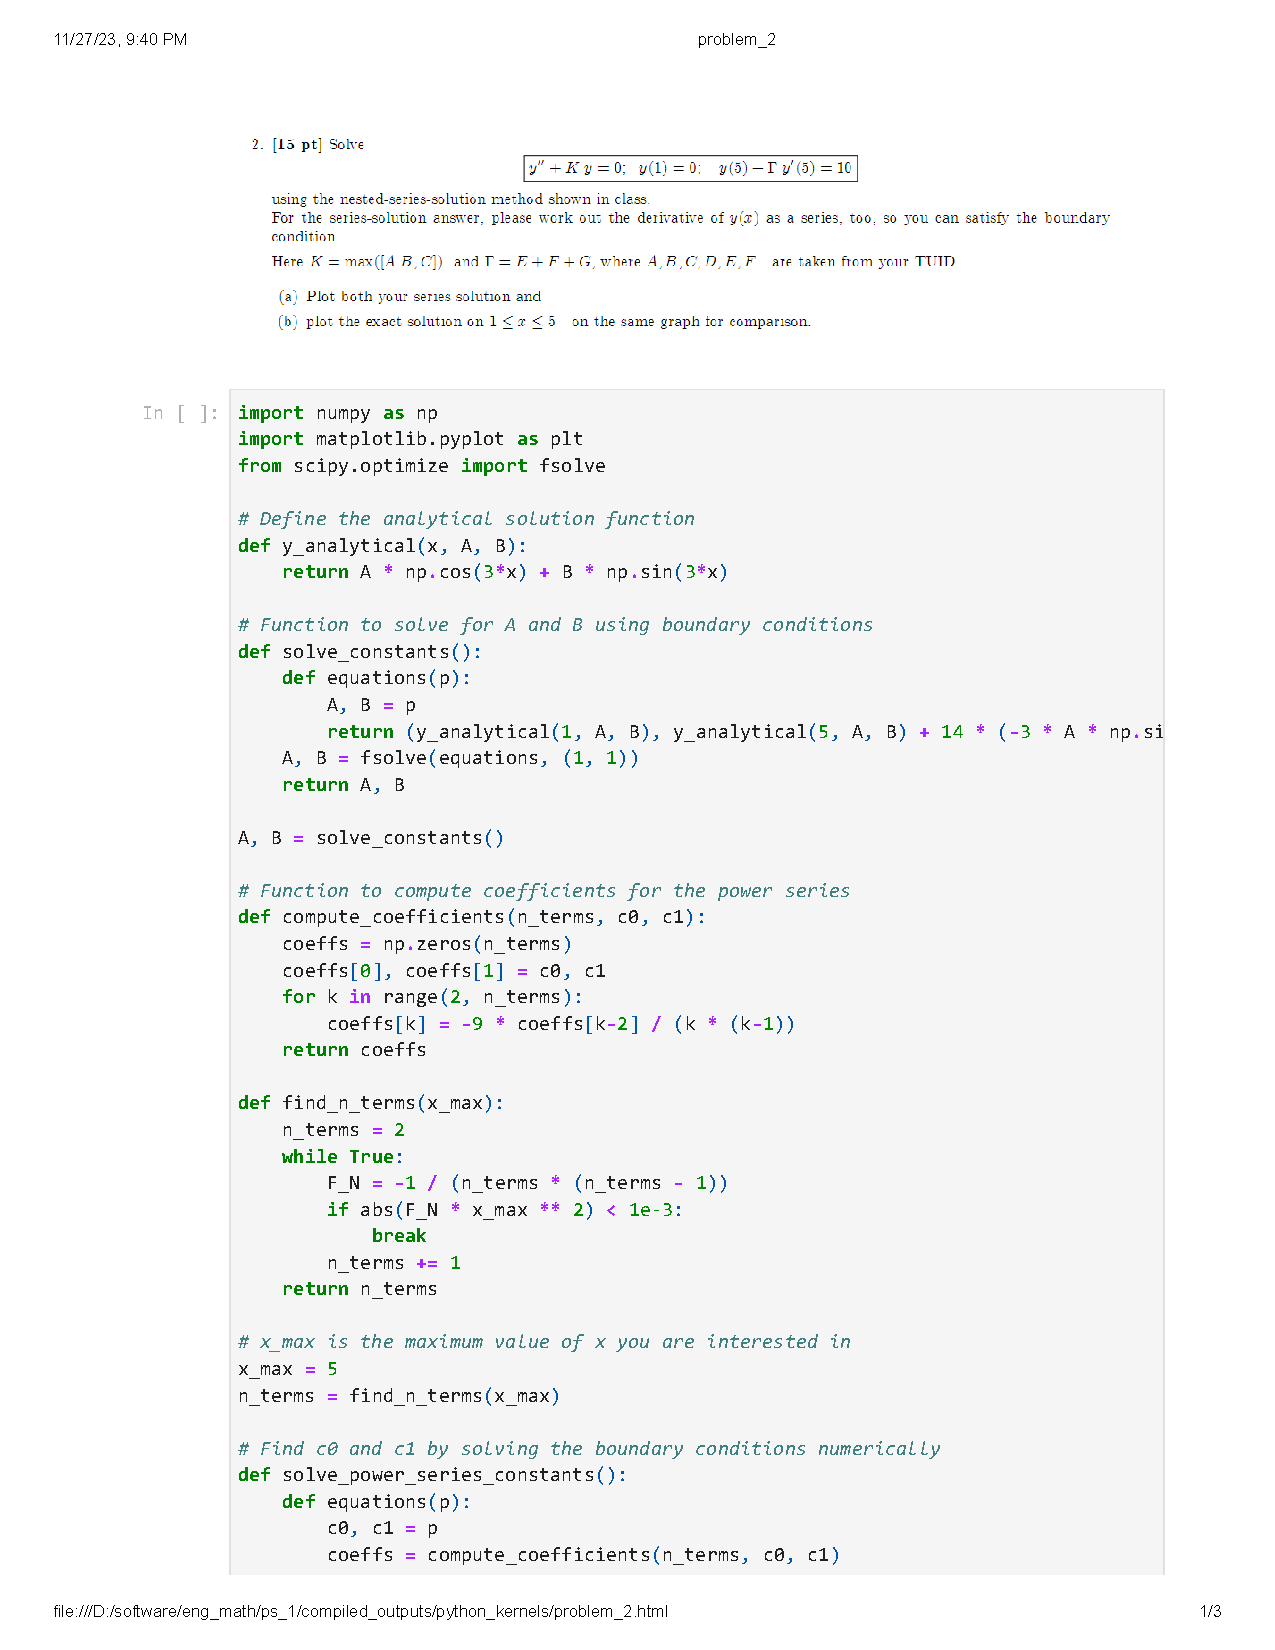
\includepdf[pages=-]{compiled_outputs/python_kernels/problem_2.pdf}
% 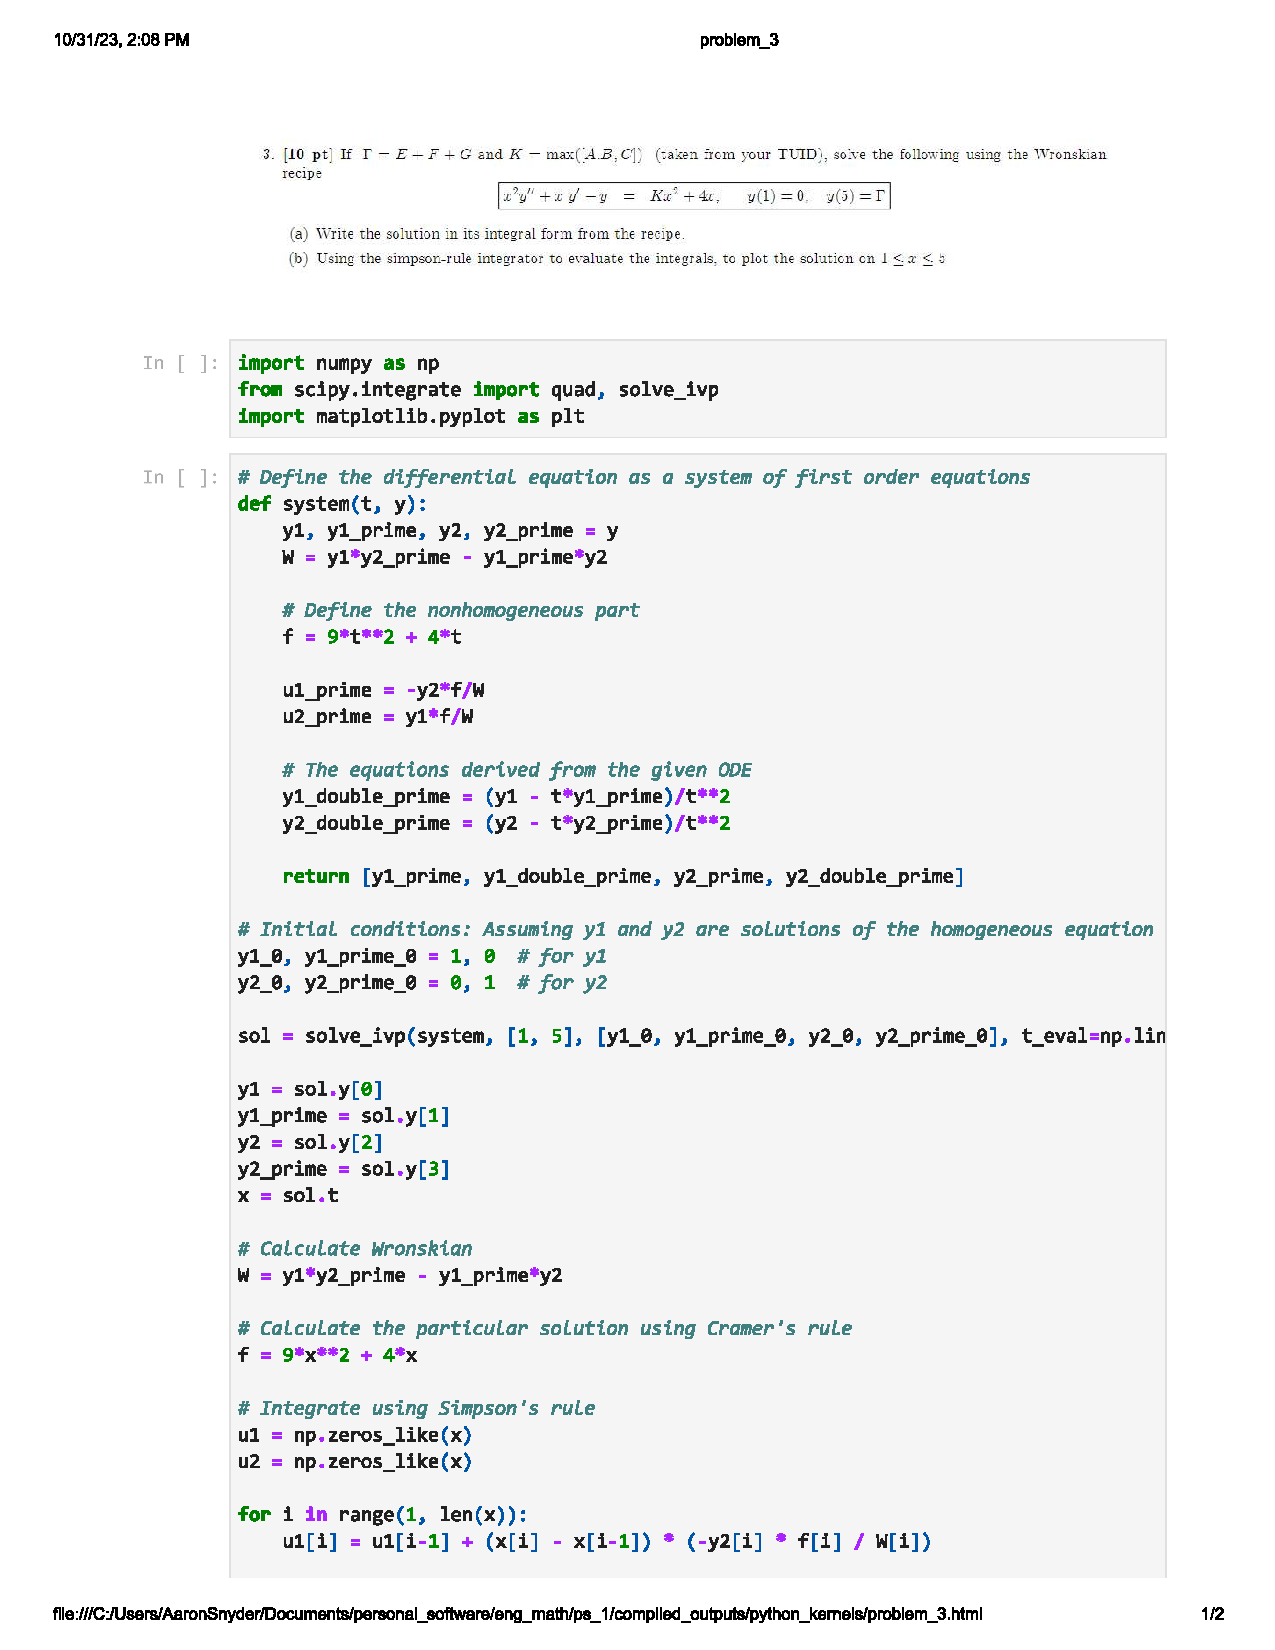
\includepdf[pages=-]{compiled_outputs/python_kernels/problem_3.pdf}
% 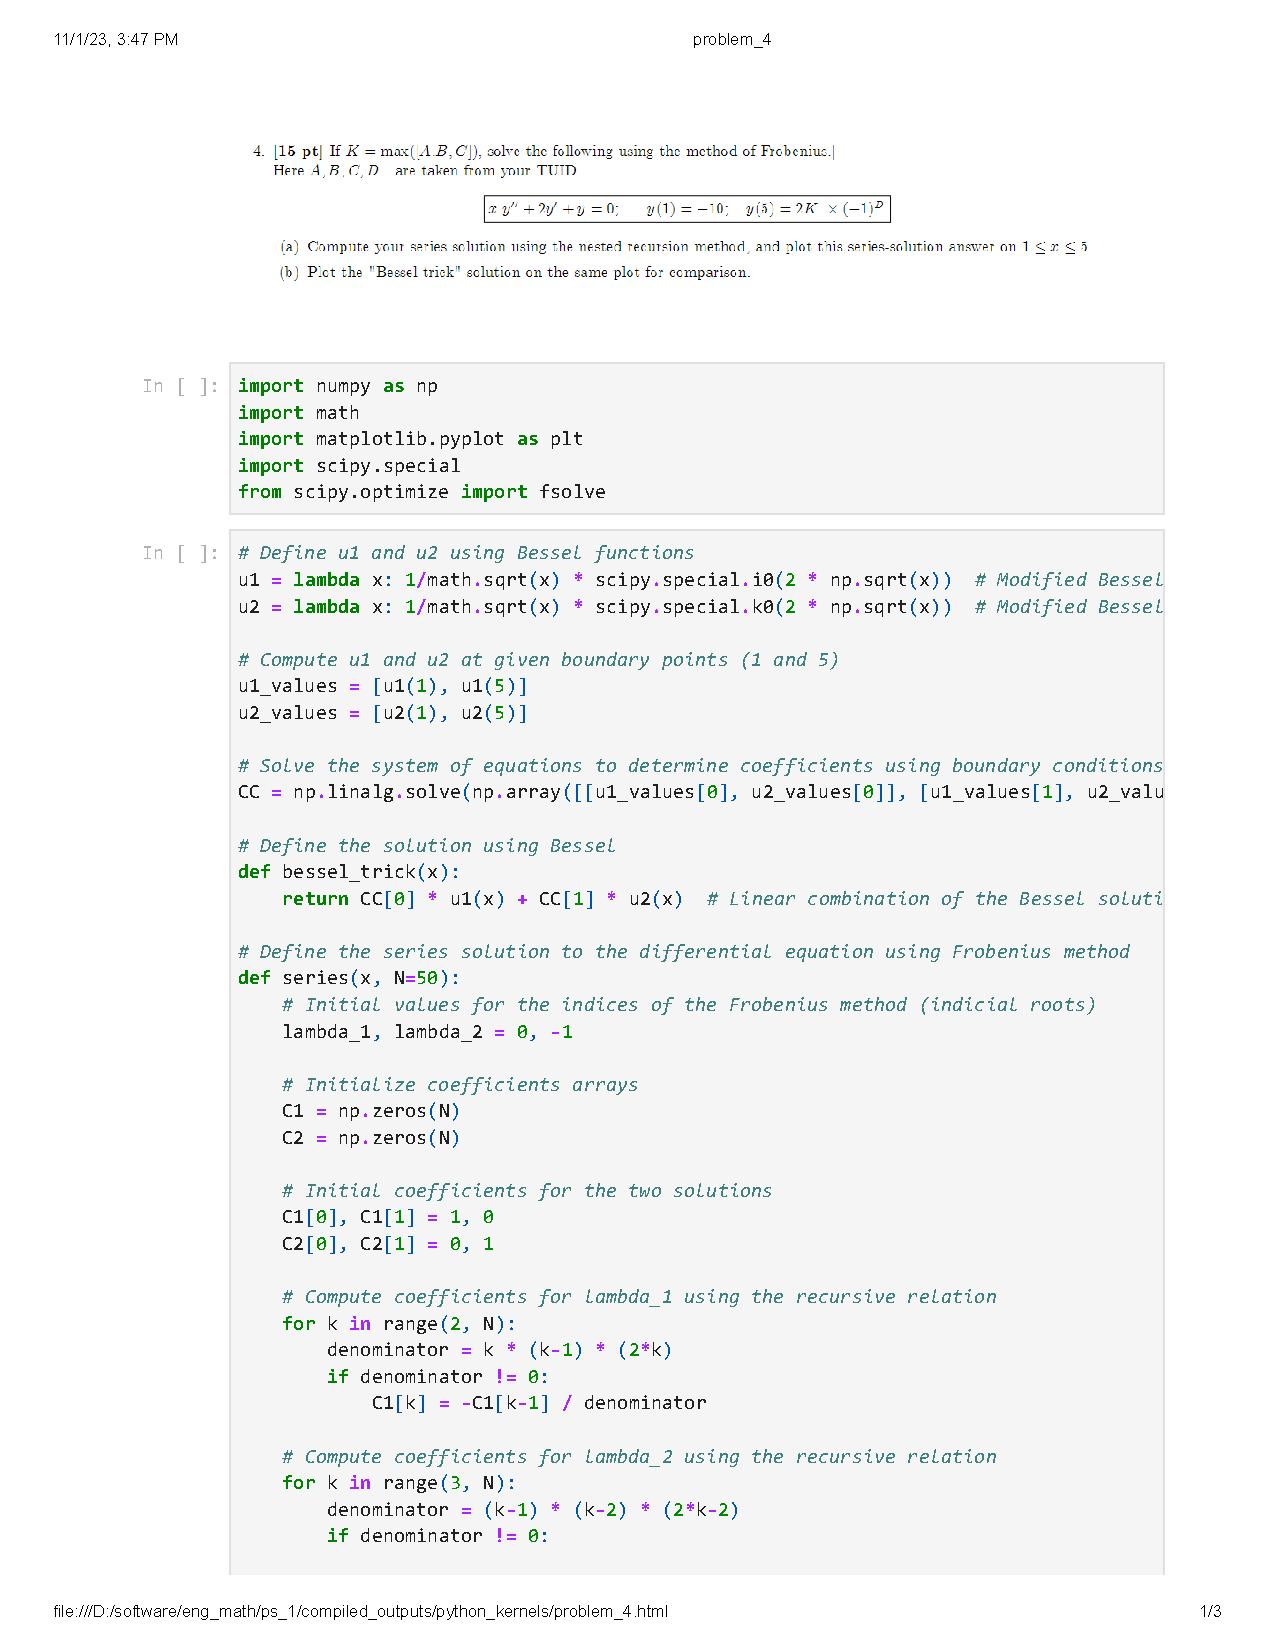
\includepdf[pages=-]{compiled_outputs/python_kernels/problem_4.pdf}

\section{MATLAB Outputs}
\begin{figure}[h]
    \centering
    \includegraphics[width=0.5\textwidth]{misc_media/Matlab-Logo.jpg}
    \caption{MATLAB Logo}  % Optional: add a caption
    \label{fig:matlab-logo} % Optional: add a label for referencing
\end{figure}

\vspace{2cm}  % Add vertical space of 2cm

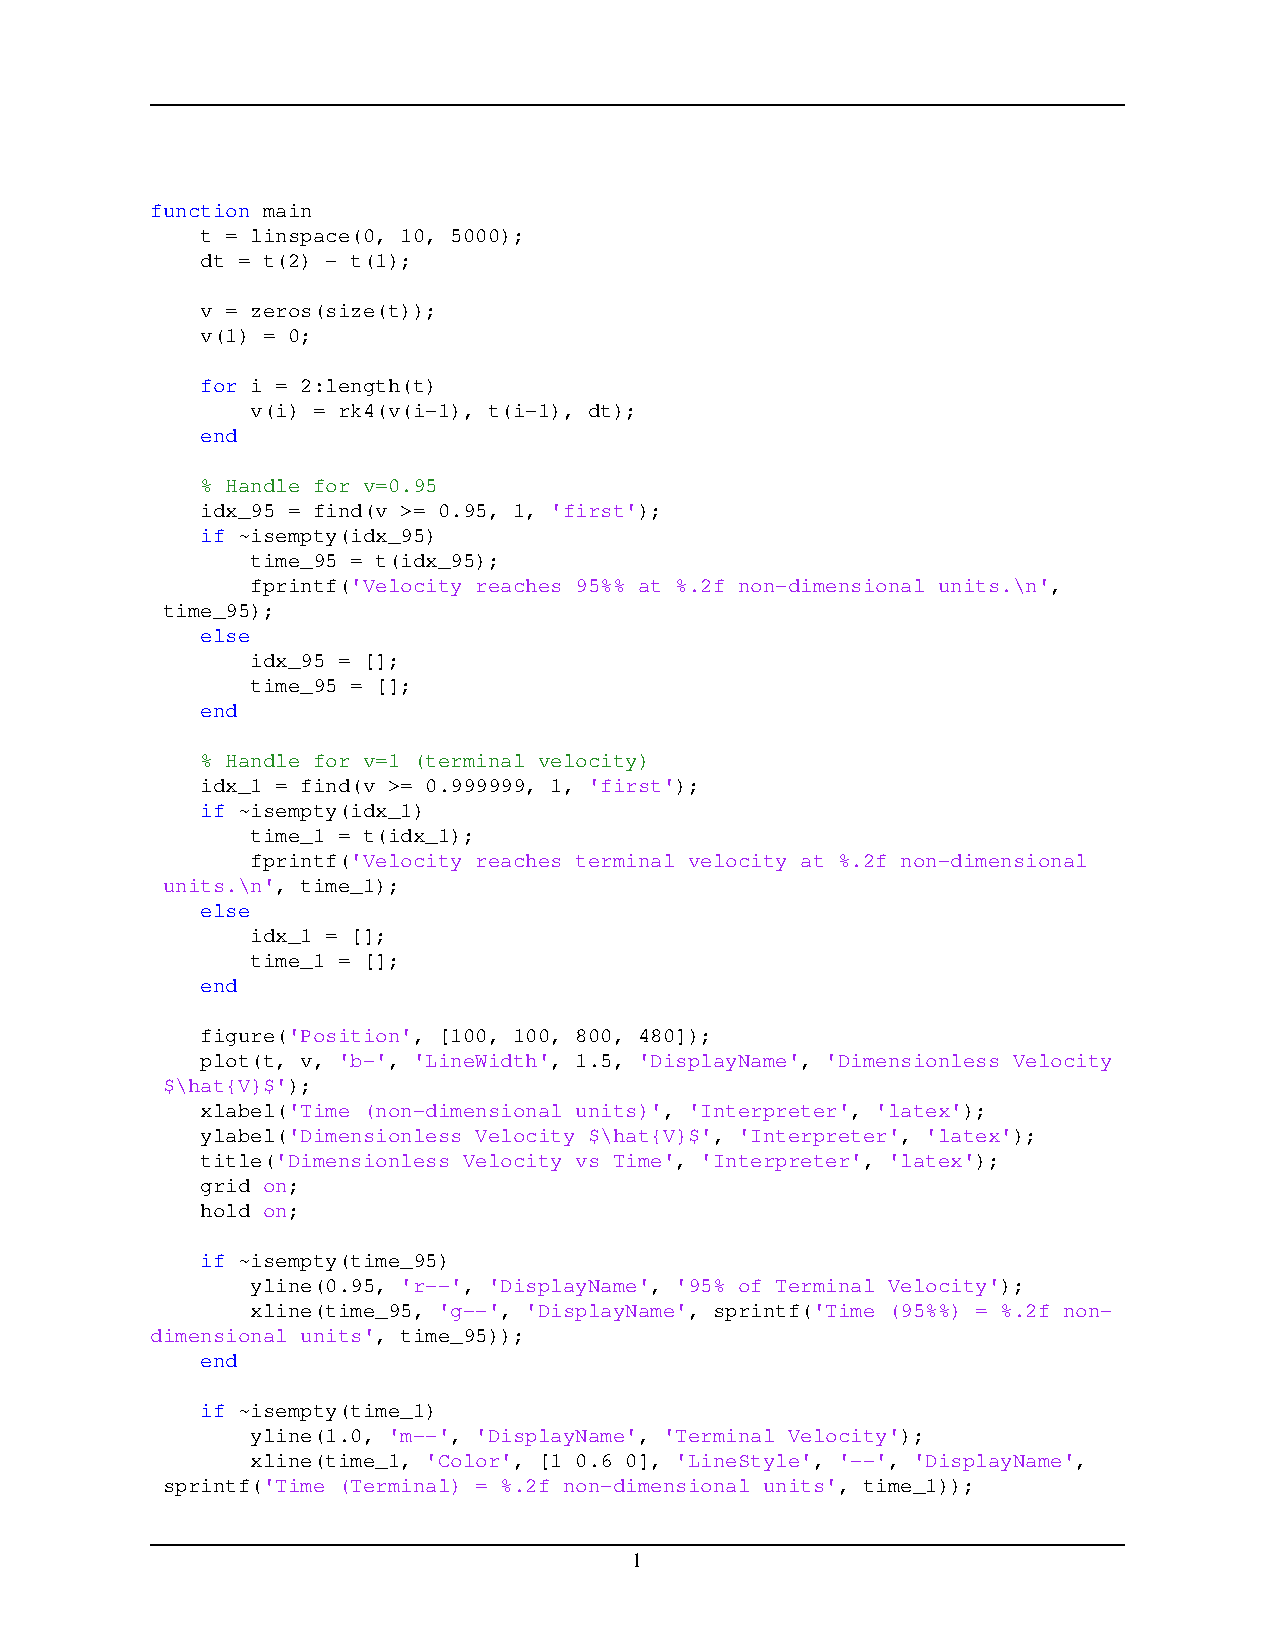
\includepdf[pages=-]{compiled_outputs/matlab_functions/problem_1.pdf}
% 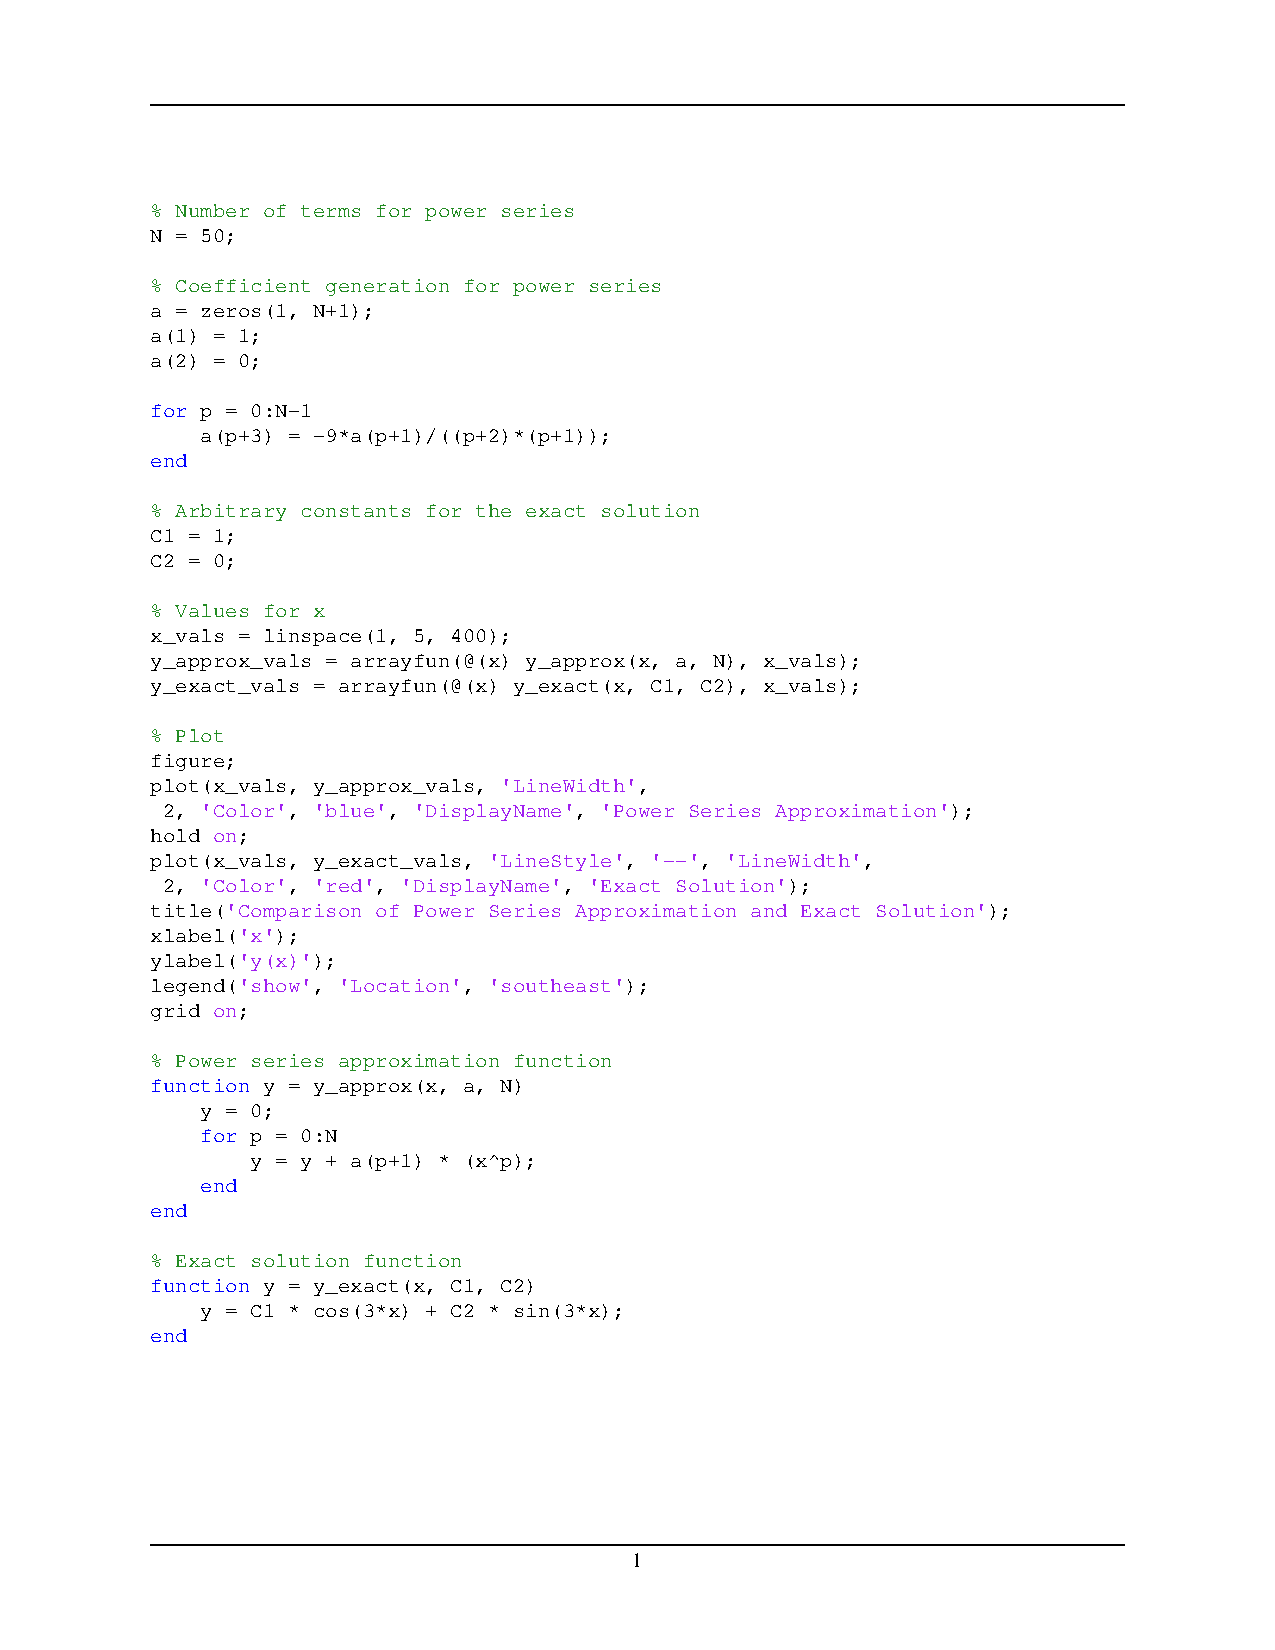
\includepdf[pages=-]{compiled_outputs/matlab_functions/problem_2.pdf}
% 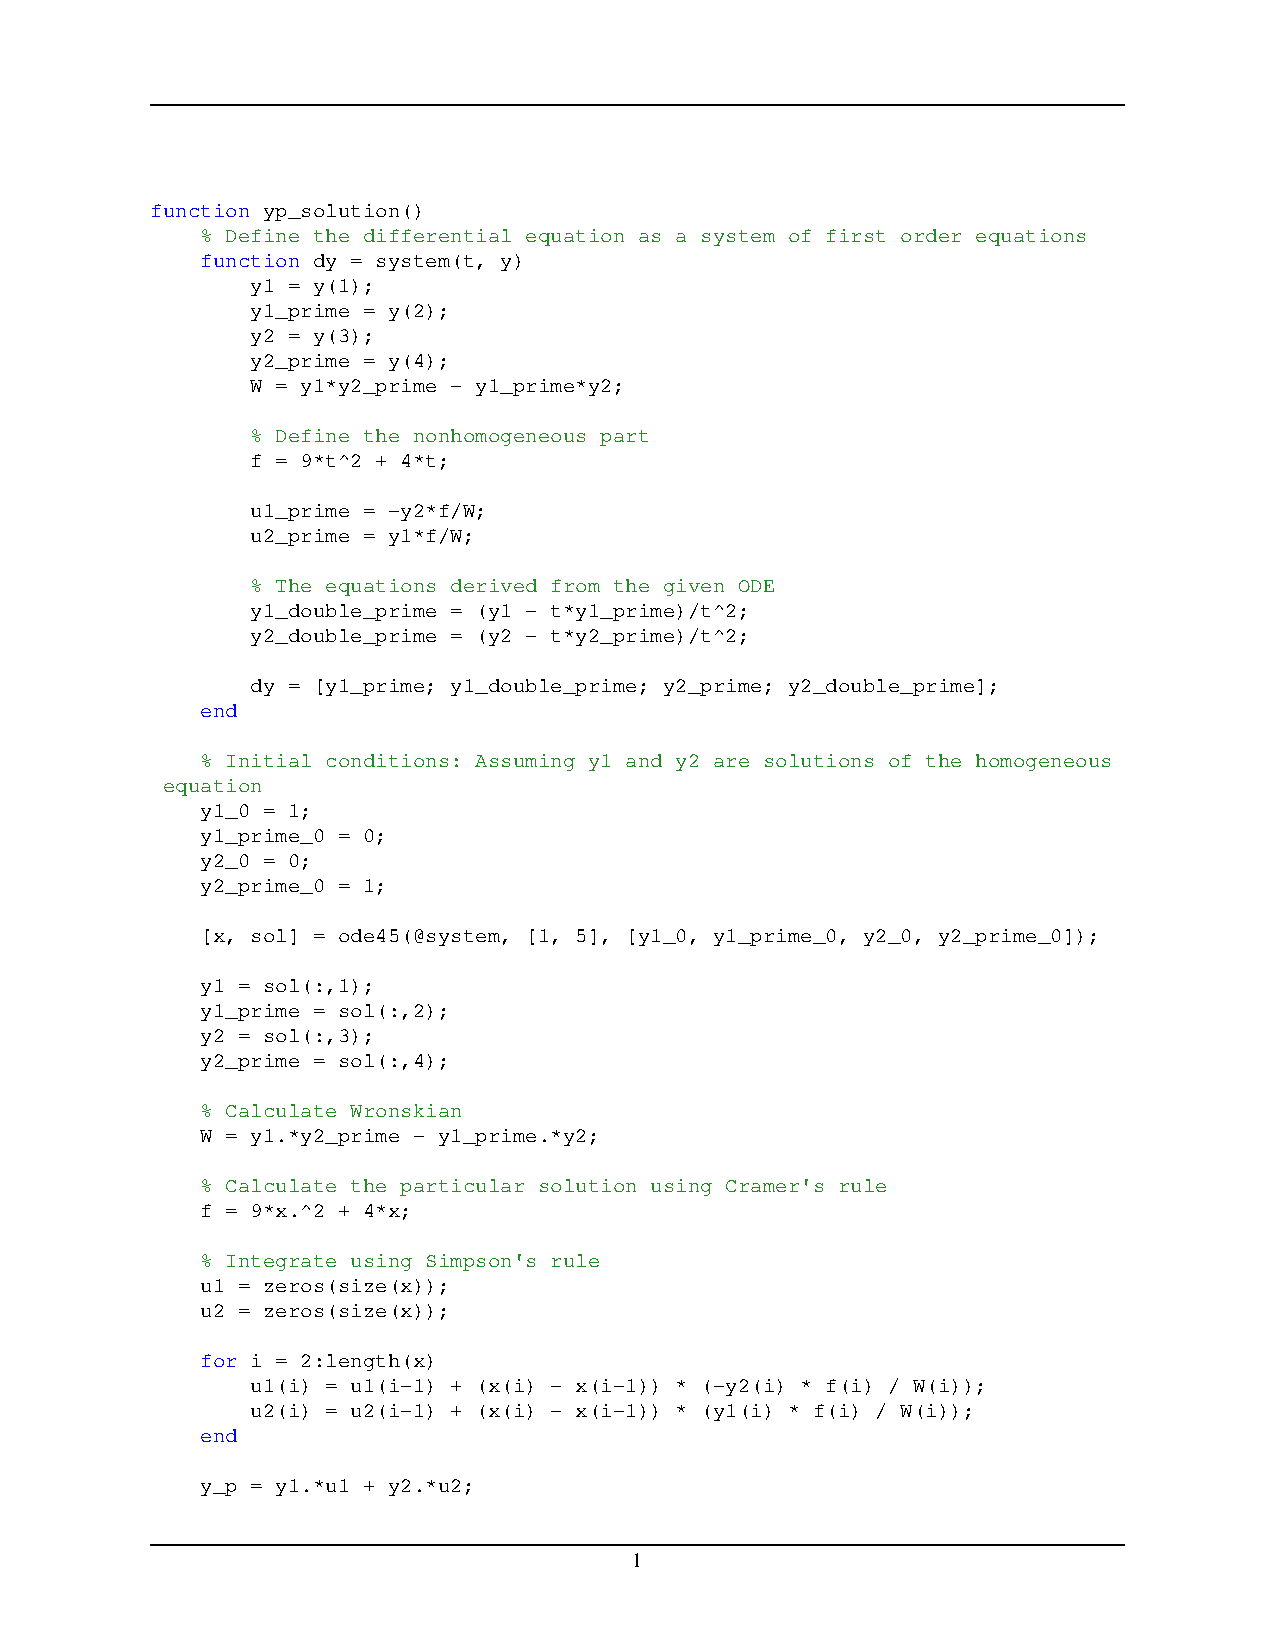
\includepdf[pages=-]{compiled_outputs/matlab_functions/problem_3.pdf}
% 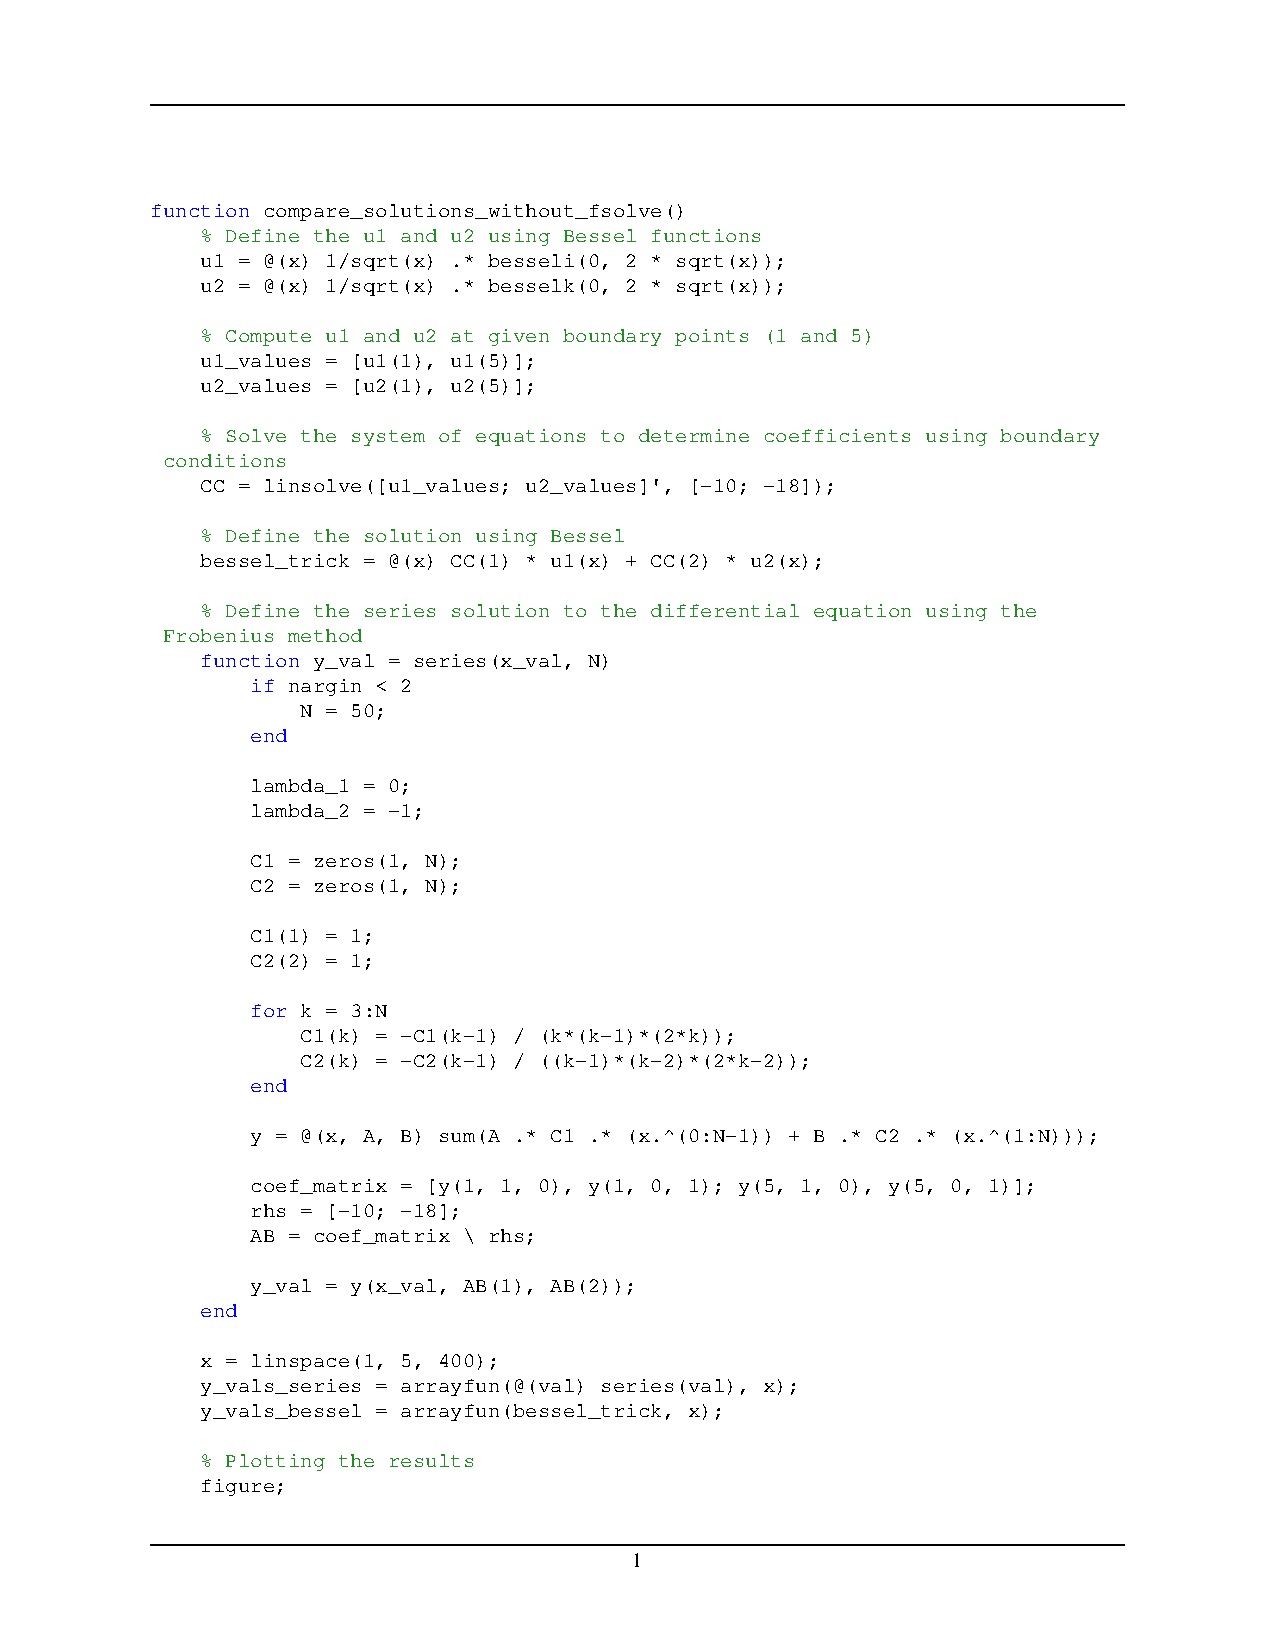
\includepdf[pages=-]{compiled_outputs/matlab_functions/problem_4.pdf}

\section{Compiled Plots}

% Uncomment the following line and correct the path if necessary
% 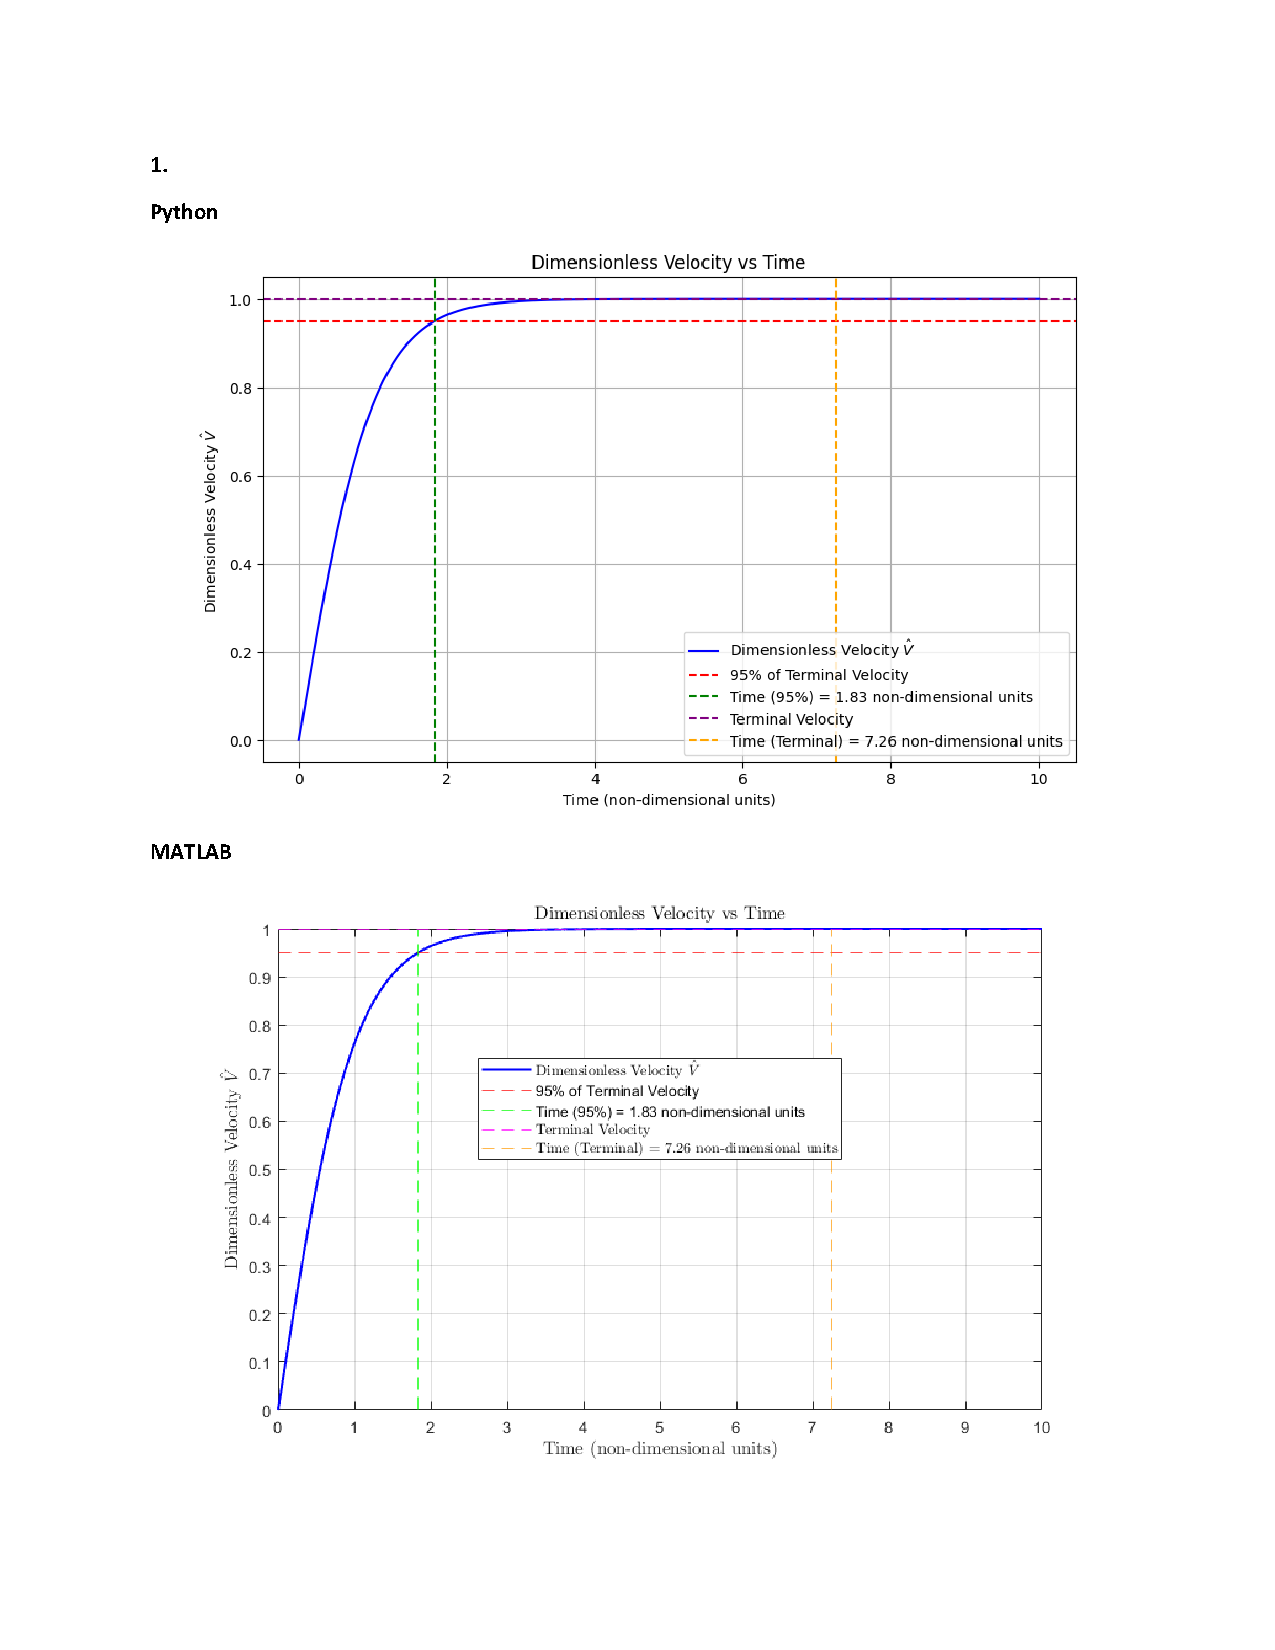
\includepdf[pages=-]{compiled_outputs/compiled_plots.pdf}

\end{document}
